\todo{Rewrite chapter introduction}

\subsection{Implementing the algorithm}

\subsubsection{Step 1: Visit}

To support the parallel visiting of URLs in one virtual machine, we had to extend Cuckoo. Support for this was added pretty quickly using tabs, but this left us with a problem to detect when a new URL was feeded to a tab\todo{See problems below}. To solve this problem, every URL is now opened in its own window.

\subsubsection{Step 2: Process}
\begin{description}
\item[on\_process\_new] sfdsfdf
\item[on\_process\_finished] sfdsfdf
\item[on\_http\_request] sfdsfdf
\item[on\_file\_write] sfdsfdf
\item[on\_file\_delete] sfdsfdf
\item[on\_registry\_set] sfdsfdf
\item[on\_registry\_delete] sfdsfdf
\item[on\_shell\_execute] sfdsfdf
\item[on\_socket\_connect] sfdsfdf
\item[on\_anomaly\_detected] sfdsfdf
\end{description}
\subsubsection{Step 3: Analyze}

To implement the analysis phase of the algorithm, a simple analyzer was written that detects process spawns below browsing contexts. Listing \todo{reffie} shows pseudo code of the analyzer.

\begin{lstlisting}
function deep_process_spawn_analyzer(graph)
    foreach vertex in graph
        if vertex.type == "process_spawned"
            if check_depth_in_graph(vertex, 0) > 1
                print "Malicious activity"
            endif
        endif
    endforeach
endfunction

function check_depth_in_graph(vertex, current_depth)
    parents = get_parents_of_vertex(vertex)
    # Actually we need only one parent
    if length_array(parents) > 0
        return check_depth_in_graph(parents[0], current_depth++)
    else
        # No more parents, we're at the root node
        return current_depth
    endif
endfunction
\end{lstlisting}

\subsubsection{Problems}
\label{99problems}
\epigraph{I've got 99 problems but Cuckoo ain't one.}{Adriaan}

\begin{itemize}
\item Out of order openen en sluiten van handles 
\item Paralellizatie problemen
\item BSON file loggen naar de host
\item Weten wanneer een nieuwe URL wordt geopend
\begin{itemize}
\item Geen TypedURLs met COM
\item COM (CrossZoneCompare, blocking Navigate met deadlock tot gevolg, )
\end{itemize}
\item Opsplitsen / linken van de data in 1 process over meerdere requests
\item Missende data door te kleine buffers en niet geimplementeerde apis in cuckoomon
\end{itemize}

\subsection{Step 4: Report}
\todo{Betere analyzer reporting in output script...}
\begin{lstlisting}
$ python cuckoo.py &
$ python utils/mass-analyse.py -g -t 22
Warning: Task with ID 22 is not yet completed; Waiting...
INFO:root:Parse log....
Analyzer 'Subprocess_from_tab': The URL 'http://malware-site.com' 
spawns a process called 'errfix.exe'.
\end{lstlisting}

\subsection{Running the PoC}
\newgeometry{left=3cm,top=0.1cm,bottom=0.1cm}
 \todo{Explain the colors of the vertices}
\begin{figure}[h]
    \centering
    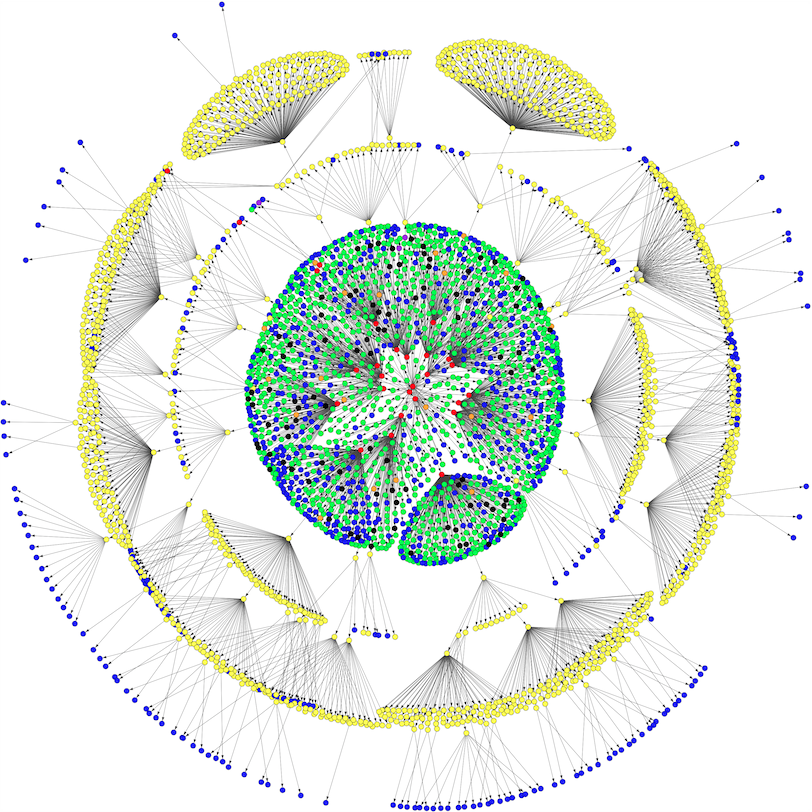
\includegraphics[width=17cm]{Images/graph2.png}
    \caption{An example of the graph}
    \label{fig:graph}
\end{figure}
\subsubsection{Step 6}
\begin{figure}[h]
    \centering
    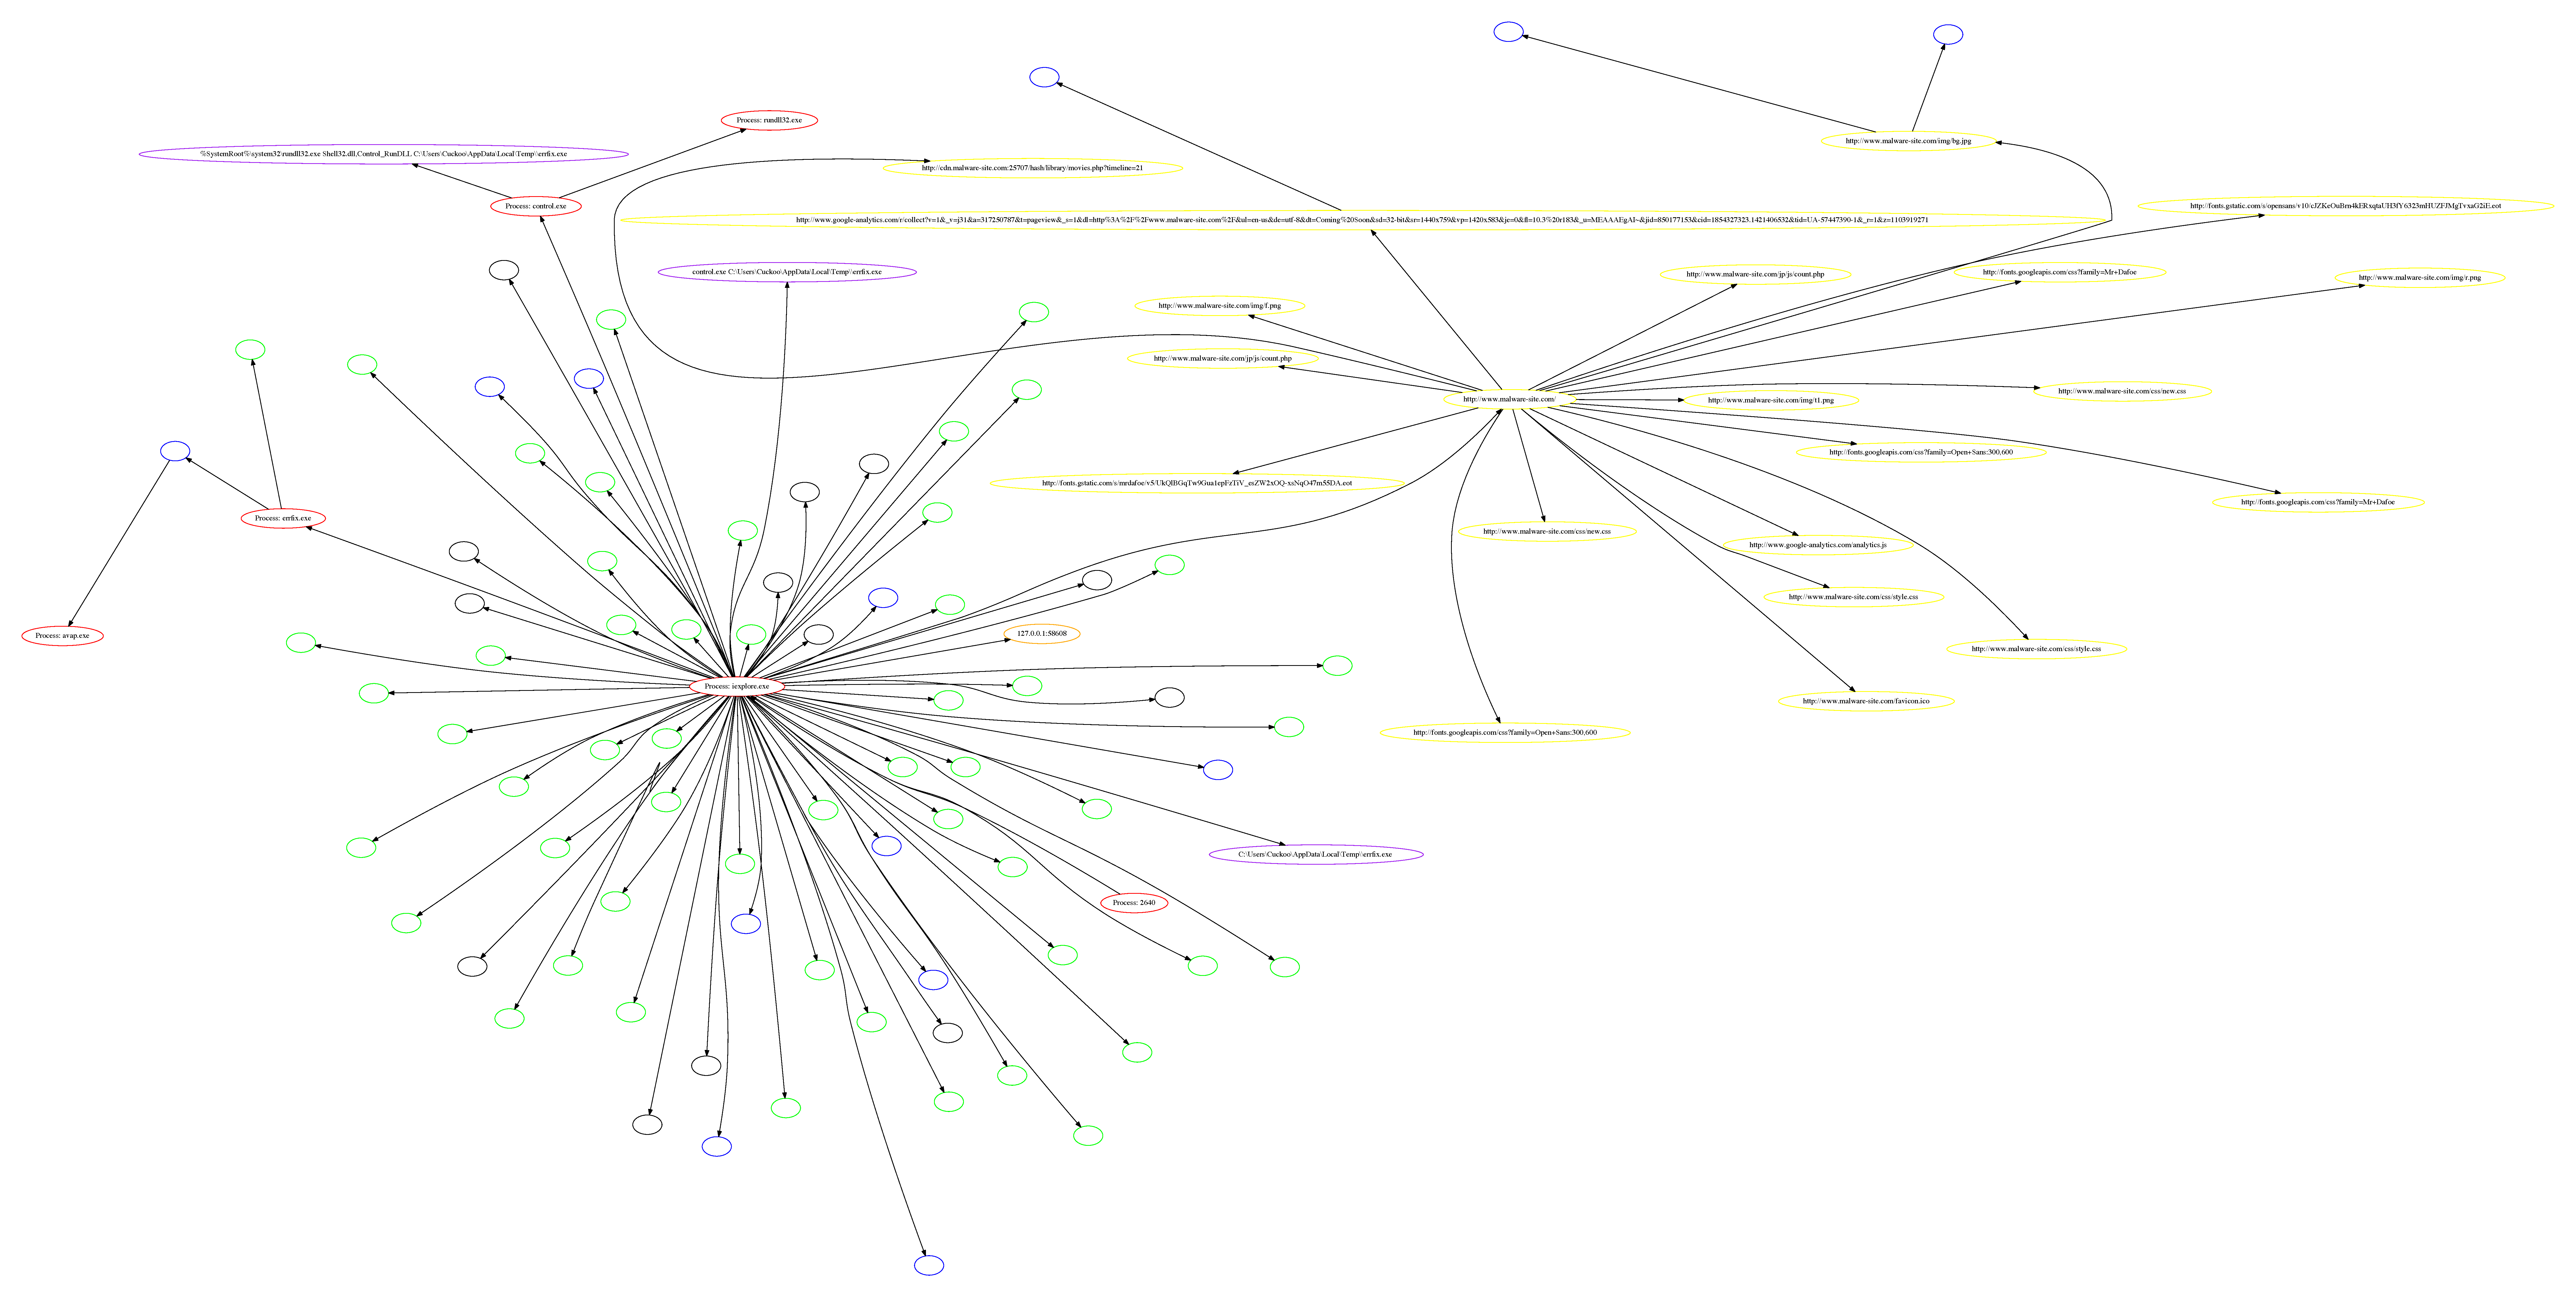
\includegraphics[width=25cm, angle=90]{Images/report_Subprocess_from_tab}
    \caption{An example of the subgraph of a single website that injected the virtual machine with malware. For clarity are only the labels of the nodes of visited URLs, involved processes and executed shell commands showed.}
    \label{fig:subgraph}
\end{figure}

\todo{Speedboost tussen Cuckoo 1.2-dev en onze wijzigingen in grafiekje zetten}

